%
% $RCSfile: layers.tex,v $
%
% Copyright (c) 2004. Christian Heller. All rights reserved.
%
% No copying, altering, distribution or any other actions concerning this
% document, except after explicit permission by the author!
% At some later point in time, this document is planned to be put under
% the GNU FDL license. For now, _everything_ is _restricted_ by the author.
%
% http://www.cybop.net
% - Cybernetics Oriented Programming -
%
% http://www.resmedicinae.org
% - Information in Medicine -
%
% @author Christian Heller <christian.heller@tuxtax.de>
%

\paragraph{Layers}
\label{layers_heading}

The \emph{Layers} pattern \cite{buschmann} is one of the most often used
principles to subdivide a system into logical levels. One famous variant contains
the three layers \emph{Presentation}, \emph{Domain Logic} and \emph{Data Source}.
Another well-known example making use of this pattern is the
\emph{Open Systems Interconnection} (OSI) reference model, defined by the
\emph{International Organization for Standardization} (ISO). Numerous books
\cite{tanenbaum2000,payer} describe this model and its protocols.

\begin{figure}[ht]
    \begin{center}
        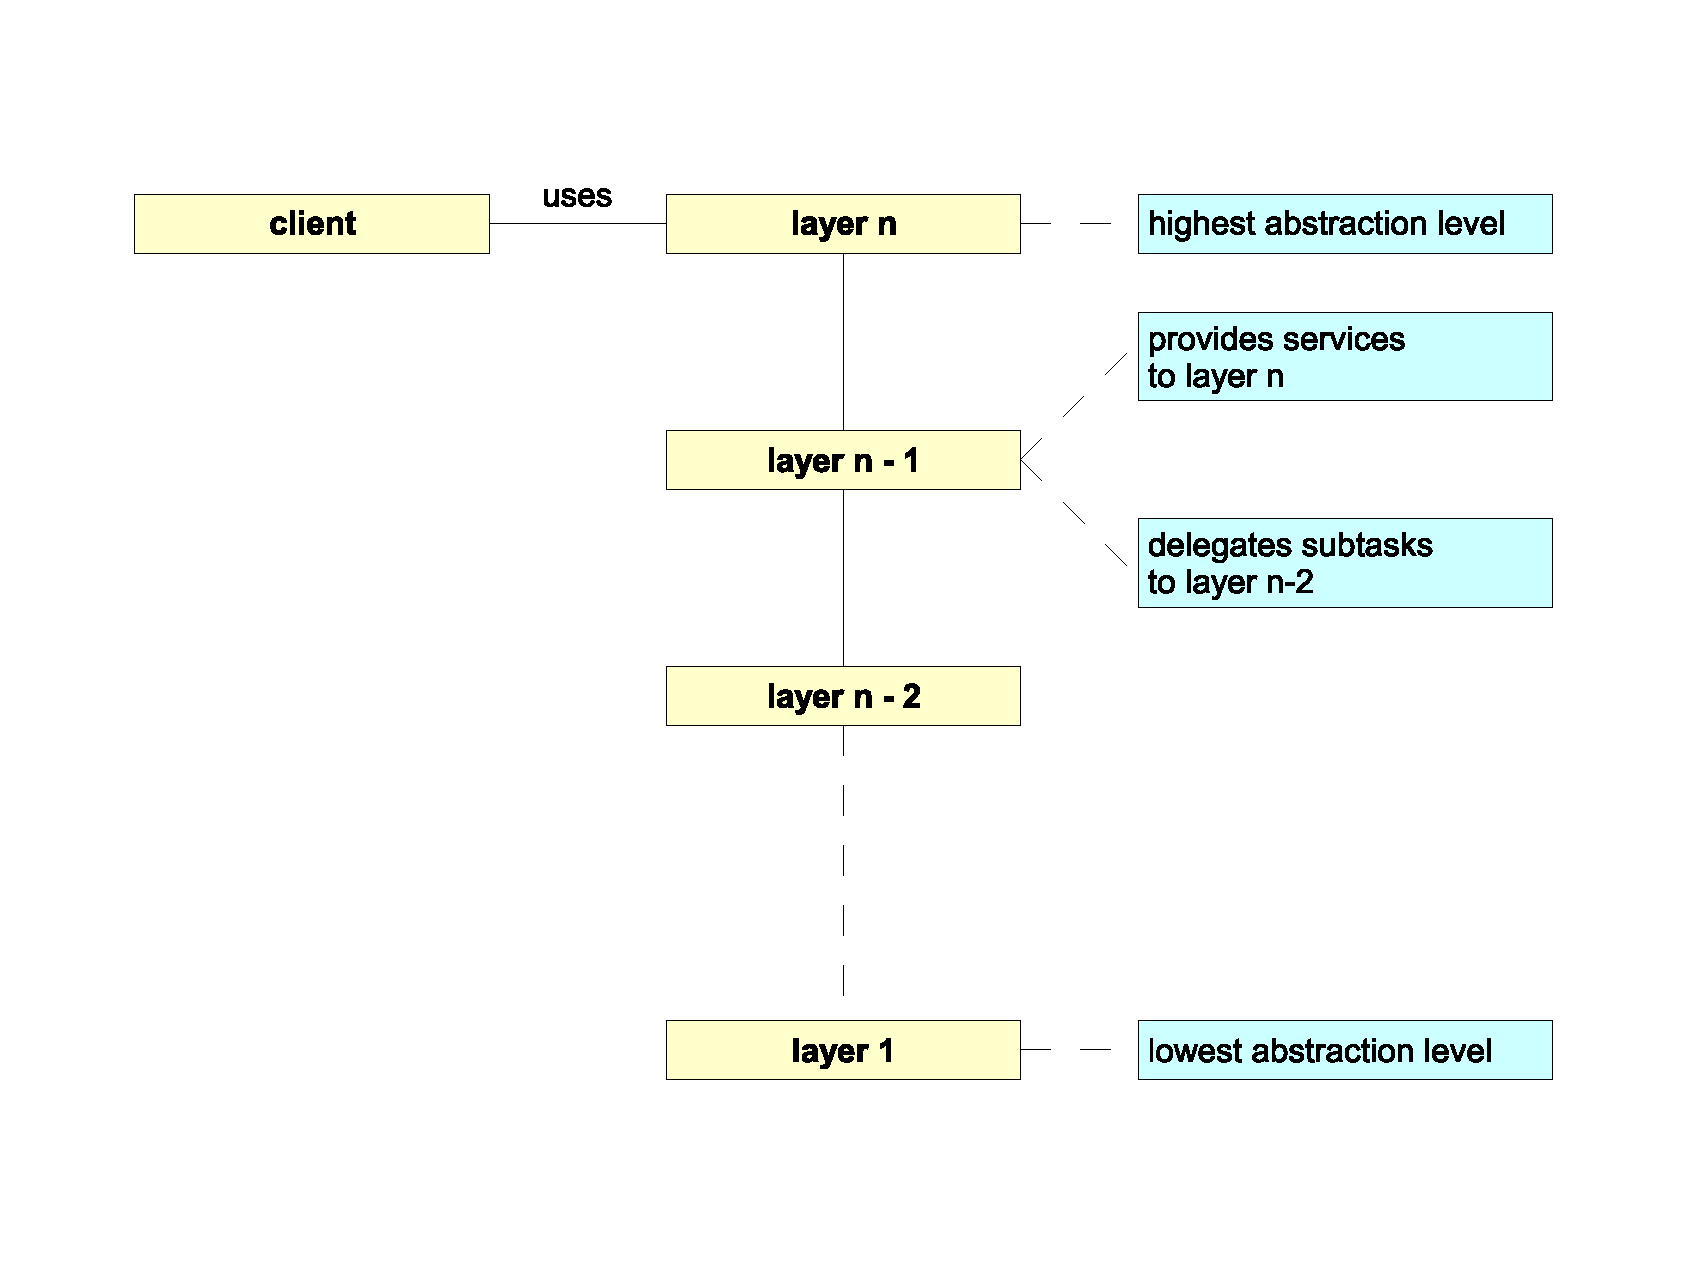
\includegraphics[scale=0.3]{vector/layers.eps}
        \caption{Layers Pattern}
        \label{layers_figure}
    \end{center}
\end{figure}

A more general illustration can be seen in figure \ref{layers_figure}. It shows
a client using the functionality encapsulated in a layer. That top-most layer
delegates subtasks to lower-level layers which are specialized on solving them.

One variant of this pattern, mentioned by Buschmann \cite{buschmann}, is the
\emph{Relaxed-Layered-System}. It permits a layer to not only use the services
of its direct base layer, but also of yet lower-situated layers. The base layer
in this case is called \emph{transparent}.
